% !TEX TS-program = pdflatexmk
%% 
%% Copyright 2026 Elsevier Ltd
%% 
%% This file is part of the 'Elsarticle Bundle'.
%% ---------------------------------------------
%% 
%% It may be distributed under the conditions of the LaTeX Project Public
%% License, either version 1.2 of this license or (at your option) any
%% later version.  The latest version of this license is in
%%    http://www.latex-project.org/lppl.txt
%% and version 1.2 or later is part of all distributions of LaTeX
%% version 1999/12/01 or later.
%% 
%% The list of all files belonging to the 'Elsarticle Bundle' is
%% given in the file `manifest.txt'.
%% 

%% Template article for Elsevier's document class `elsarticle'
%% with numbered style bibliographic references
%% SP 2008/03/01

\documentclass[preprint,12pt, a4paper]{elsarticle}


\usepackage{amssymb}
\usepackage{hyperref}
% \setlength{\parindent}{0pt}
\usepackage{booktabs}
\usepackage{array}
\usepackage{float}
\usepackage{pdfcomment}
\usepackage{amsmath}
\usepackage{cancel}
\usepackage{graphicx}
\usepackage{subcaption}
\usepackage{minted}
\usepackage{makecell}
\usepackage{xcolor}
\usepackage{multicol}
\usepackage{listings}
\usepackage{algorithm}
\usepackage{algpseudocode}
\usepackage{caption}
\usepackage{enumitem}
%% The amsthm package provides extended theorem environments
%% \usepackage{amsthm}

\usepackage[margin=1.0in]{geometry}


%% The lineno packages adds line numbers. Start line numbering with
%% \begin{linenumbers}, end it with \end{linenumbers}. Or switch it on
%% for the whole article with \linenumbers.
% \usepackage{lineno}
% \linenumbers

\journal{SoftwareX}

\begin{document}
\renewcommand{\labelenumii}{\arabic{enumi}.\arabic{enumii}}

\begin{frontmatter}


\title{\textsc{CodeJeNN}: A simple C\texttt{++} neural network generator for physics applications}


\author[SDSU]{Jay Arcities}
\author[SDSU]{Pavel Popov}
\author[NRL]{Eric J. Ching}
\author[NRL]{Kamal Viswanath}
\author[NRL]{Ryan F. Johnson}

\address[SDSU]{San Diego State University, Aerospace Engineering Department, San Diego, CA 92182}
\address[NRL]{U.S. Naval Research Laboratory, Laboratories of Computational Physics and Fluid Dynamics, Washington, DC 20375}

% \textbf{Before you begin: DELETE THIS SECTION BEFORE SUBMISSION}

% \begin{itemize}
% 	\item This template is for an original SoftwareX article. If you are submitting an update to a software article that has already been published, please use the software update template from the Guide for Authors.
%     \item The format of a software article is very different to a traditional research article. To help you write yours, we have created this template. We will only consider software articles submitted using this template. Any submission that deviates widely will likely face desk rejection.
%     \item It is mandatory to publicly share the code / software referred to in your software article. You’ll find information on our software sharing criteria in the SoftwareX Guide for Authors.  
%     \item It’s important to consult the Guide for Authors when preparing your manuscript; it highlights mandatory requirements and is packed with useful advice. Here are some key ones (please read):

    
%     \begin{itemize} 
%     	\item We only accept GitHub repositories within Metadata Tables. This is required for forking to our SoftwareX repository if your paper is published. We are unable accept other repositories.
%         \item GitHub repositories must have a well-documented README.md file, and a Licence.txt file. Your paper will be returned if these are missing.
%         \item Our word limit is 4,000 words. Please focus your paper on the software and place supporting information into your GitHub repository README.md file.
%         \item We require the five (5) main templated sections outlined below. Your paper will be returned or rejected if these are missing.
% 	\end{itemize}
% \end{itemize}

\begin{abstract}
%% Text of abstract 
% Ca. 100 words
Machine learning has shown speedups for numerical methods in physics applications, but integrating Python-based libraries into high-performance C++ solvers creates performance bottlenecks. We present \textsc{CodeJeNN}, which bridges this gap by auto-generating self-contained C++ code from trained Keras models for inference. This eliminates external dependencies through minimal inlined functions, allowing seamless integration into existing frameworks. We describe the Keras-to-C++ workflow, supported architectures, and limitations. \textsc{CodeJeNN} is demonstrated through inference benchmarks against Keras (eager and JIT modes) and a CFD test case modeling viscosity in a hydrogen-air mixing layer, showing speedups without sacrificing accuracy.
\end{abstract}

\begin{keyword}
%% keywords here, in the form: keyword \sep keyword
Deep Learning \sep Computational Physics \sep Inference \sep Code Generation \sep Neural Networks

\end{keyword}

\end{frontmatter}

%\linenumbers

\begin{table}[!h]
\begin{tabular}{|l|p{6.5cm}|p{6.5cm}|}
\hline
\textbf{Nr.} & \textbf{Code metadata description} & \textbf{Please fill in this column} \\
\hline
C1 & Current code version & v1.0 \\
\hline
C2 & Permanent GitHub link to code/repository used for this code version & \url{https://github.com/jarcities/codejenn} \\
\hline
C3 & Legal Code License & NRL Open License Agreement \\
\hline
C4 & Code versioning system used & Git \\
\hline
C5 & Software code languages, tools, and services used & Python 3.12, C\texttt{++}23 \\
\hline
C6 & Compilation requirements, operating environments \& dependencies & Keras 3, Anaconda Distribution \\
\hline
C7 & If available Link to developer documentation/manual & \url{https://github.com/jarcities/codejenn/readme.md} \\
\hline
C8 & Support email for questions & jarcities@sdsu.edu \\
\hline
\end{tabular}
\caption{Code metadata}
\label{} 
\end{table}

\let\svthefootnote\thefootnote\let\thefootnote\relax\footnotetext{\\ \hspace*{25pt}DISTRIBUTION STATEMENT A. Approved for public release. Distribution is unlimited.}\addtocounter{footnote}{-1}\let\thefootnote\svthefootnote

\section{Motivation and Significance}
Machine learning has shown promise when integrated with numerical schemes for partial differential equations (PDEs), enabling research in data-driven preconditioners \cite{hausner_learning_2024, li_learning_2023}, surrogate constitutive models \cite{fuhg_review_2025}, and physics-informed neural networks \cite{raissi_physics-informed_2019, zhao_comprehensive_2024, cai_physics-informed_2021}. In computational fluid dynamics (CFD), neural networks are applied to accelerate simulations, turbulence modeling, and reduced order models \cite{vinuesa_enhancing_2022}. Modern neural network architectures are accessible through high-level libraries like \textsc{ONNX} \cite{bai_onnx_2019}, TensorFlow \cite{martin_abadi_tensorflow_2015}, Keras \cite{chollet_keras_2015}, and \textsc{PyTorch} \cite{ansel_pytorch_2024}. However, speed and accuracy are critical during inference. Most physics solvers are written in compiled languages (Fortran, C++, etc.) for better resource control, while ML libraries are primarily Python-based. This disparity often adds computational overhead. Furthermore, integrating complex ML architectures into established solvers often requires significant implementation effort and experimentation.

The gap between ML libraries and compiled solvers often forces researchers to rely on framework-provided C++ APIs, which can be incompatible with established parallelization and vectorization codes. Delegating tensor operations to external APIs limits optimization and the efficient use of computing resources. Bati and Bryngelson \cite{bati_rosenna_2024} developed \textsc{RoseNNa}, a \textsc{Fortran}-based encoder that generates executable code for MLPs and RNNs from \textsc{ONNX} models. We developed \textsc{CodeJeNN}, a C++-based encoder that generates standalone code for trained Keras models. \textsc{CodeJeNN} produces all supporting activation and propagation functions in plain C++, allowing users to optimize source code directly without external dependencies like \textsc{Lapack} or \textsc{Eigen}. 

\textsc{CodeJeNN} is designed to be extensible and repeatable. If support for a particular architecture is not already available, the source code is structured to allow an LLM to generate only the required logic for that architecture. This provides a non-invasive approach to extending the framework while minimizing token consumption and reducing the effort required to experiment with new architectures.

The remainder of the paper is structured as follows: Section 2 covers neural network principles; Section 3 describes the \textsc{CodeJeNN} architecture and compatibility; Section 4 demonstrates the software through inference speed benchmarks and a CFD viscosity modeling case using Wilke's model \cite{wilke_viscosity_1950}; and Section 5 discusses the broader impact of \textsc{CodeJeNN}, including its extensibility, potential applications, and future development.

\section{Machine Learning Background}
A neural network is a surrogate model used to approximate complex mappings from training data. \textsc{CodeJeNN} generates code for multi-layer perceptrons (MLPs) and convolutional neural networks (CNNs). In an MLP, each layer performs an affine transformation using weights $\mathbf{w}$ and biases $\mathbf{b}$, followed by an activation function $\mathbf{\sigma}$ to introduce non-linearity, as shown in Eq. \ref{eq_affine_trans}. A typical MLP schematic is shown in Fig. \ref{fig:mlp_schematic}.
\begin{gather}\label{eq_affine_trans}
    \mathbf{a} = \mathbf{\sigma}\left(\mathbf{w}^T \mathbf{x} + \mathbf{b}\right)
\end{gather}

\begin{figure}[h!]
    \centering
    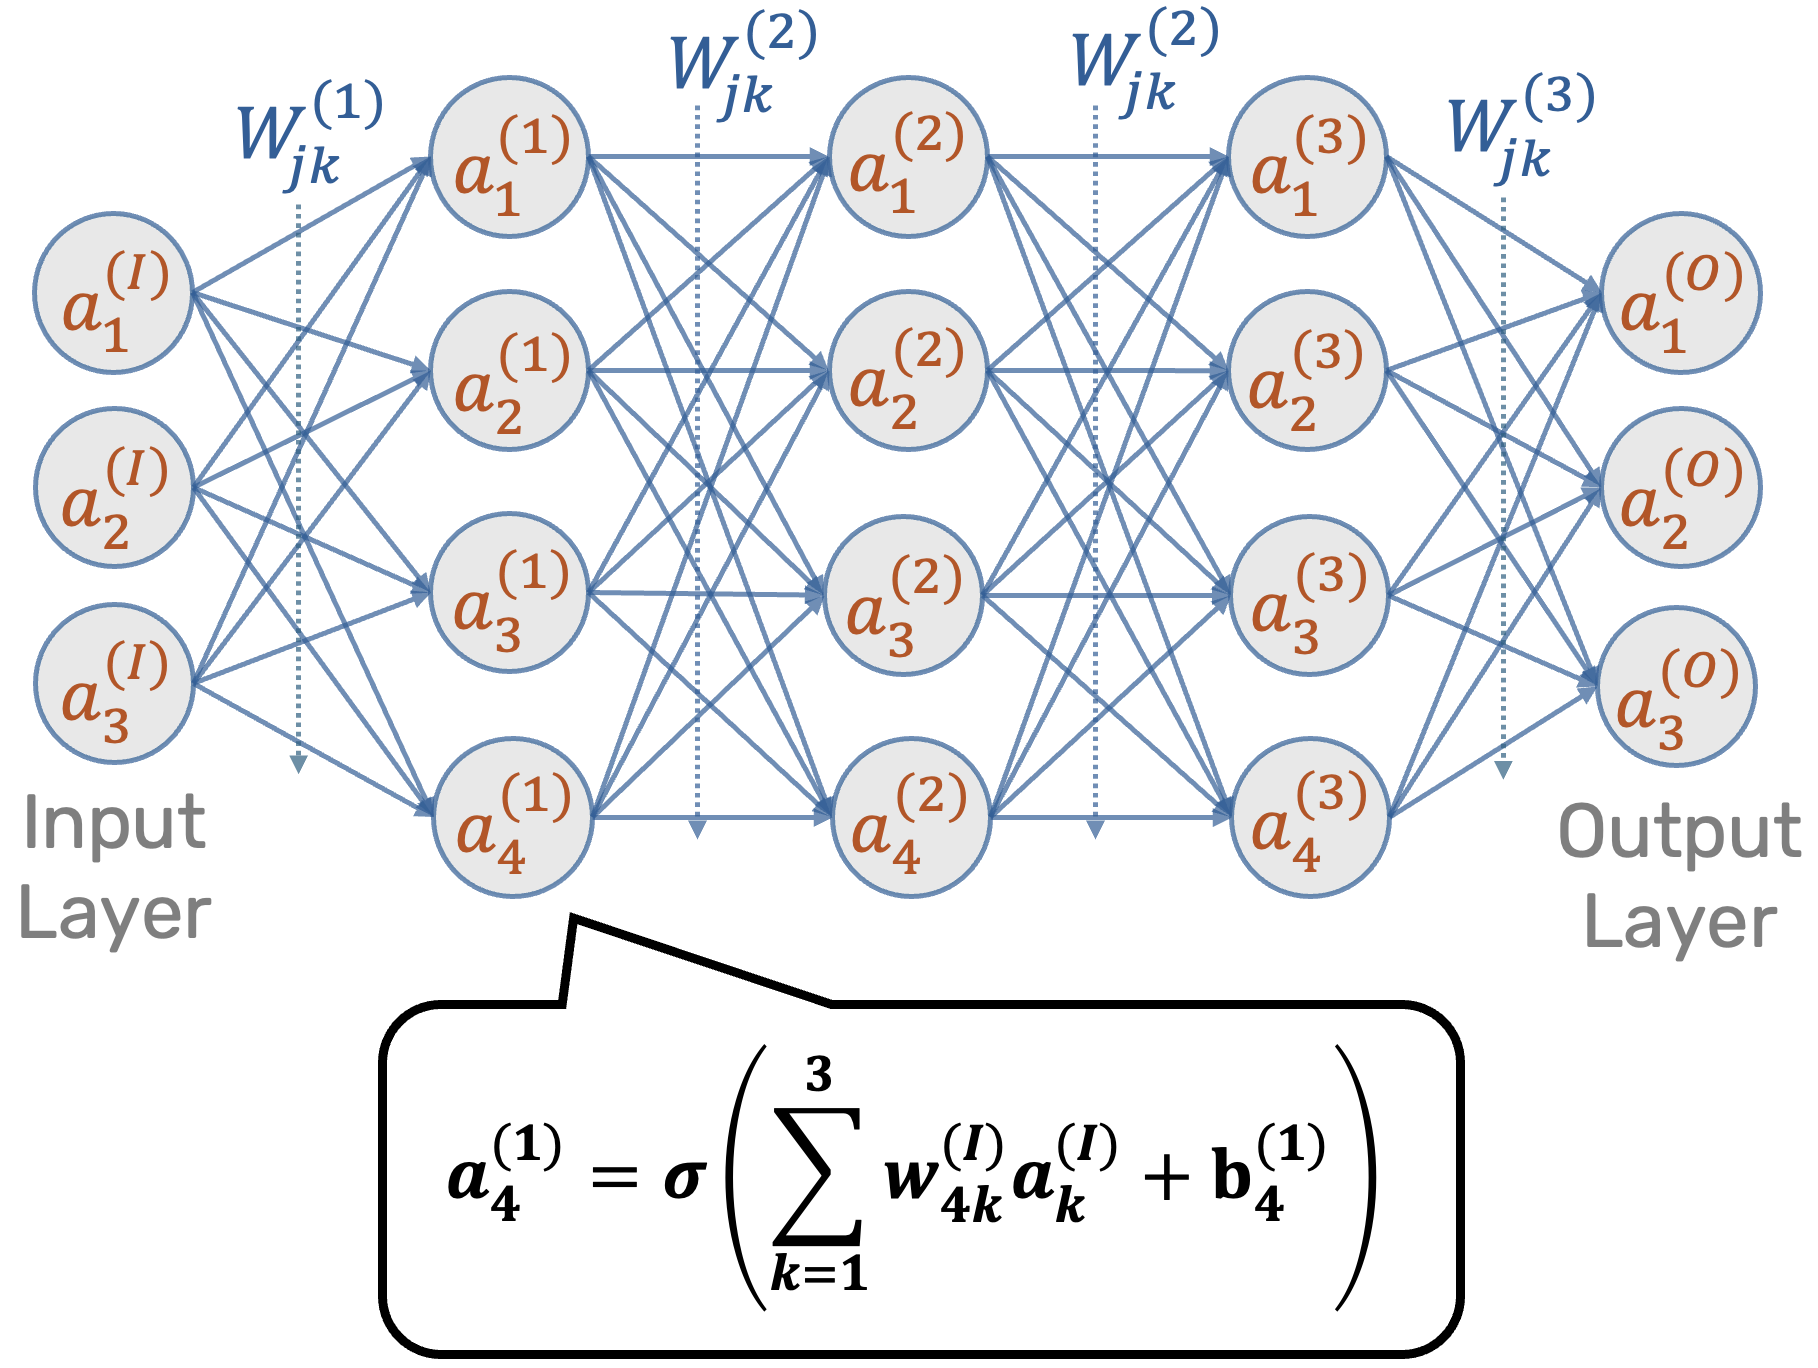
\includegraphics[width=0.45\linewidth]{figures/mlp_schematic.png}
    \caption{Schematic of a feedfoward network (MLP), where $a$ is the output from a given neuron, $w_i^{jk}$ is the specific weight sent to that neuron given the edge. Superscript defines which layer, and subscript defines which neuron in that layer. The propagation step equation for $a^{(1)}_4$ is shown in the message box.}
    \label{fig:mlp_schematic}
\end{figure}

CNNs extend this formulation using kernels to extract spatial features from multi-channel inputs:
\begin{gather}
    Y_{c_{out}, i, j} =
    \sum_{c_{in}}
    \sum_{m}
    \sum_{n}
    K_{c_{out}, c_{in}, m, n} \,
    X_{c_{in}, i+m, j+n}
    + b_{c_{out}},
    \label{eq_conv_filter_eq}
\end{gather}
Here, $c_{out}$ and $c_{in}$ are the input and output channel index of the filter, $m$ and $n$ are the spatial indices in the filter, $i$ and $j$ are the indices of the input data, and $K$ is the filter. In Eq. \ref{eq_conv_filter_eq}, the CNN layer output $Y_{c_{\text{out}}, i, j}$ is computed as a weighted combination of local input regions across all input channels, producing feature maps that capture local spatial patterns. A channel is the resulting map/matrix/image of a filter or pooling operation. A schematic of a CNN with one convolutional kernel (three filters) and two pooling layers is shown in Fig. \ref{fig:cnn_schematic}. The structural differences highlighted when comparing Fig.~\ref{fig:mlp_schematic} and Fig.~\ref{fig:cnn_schematic} illustrate the diversity of machine-learned architectures and underlines their complexity in implementation in existing codebases.

\begin{figure}[h!]
    \centering
    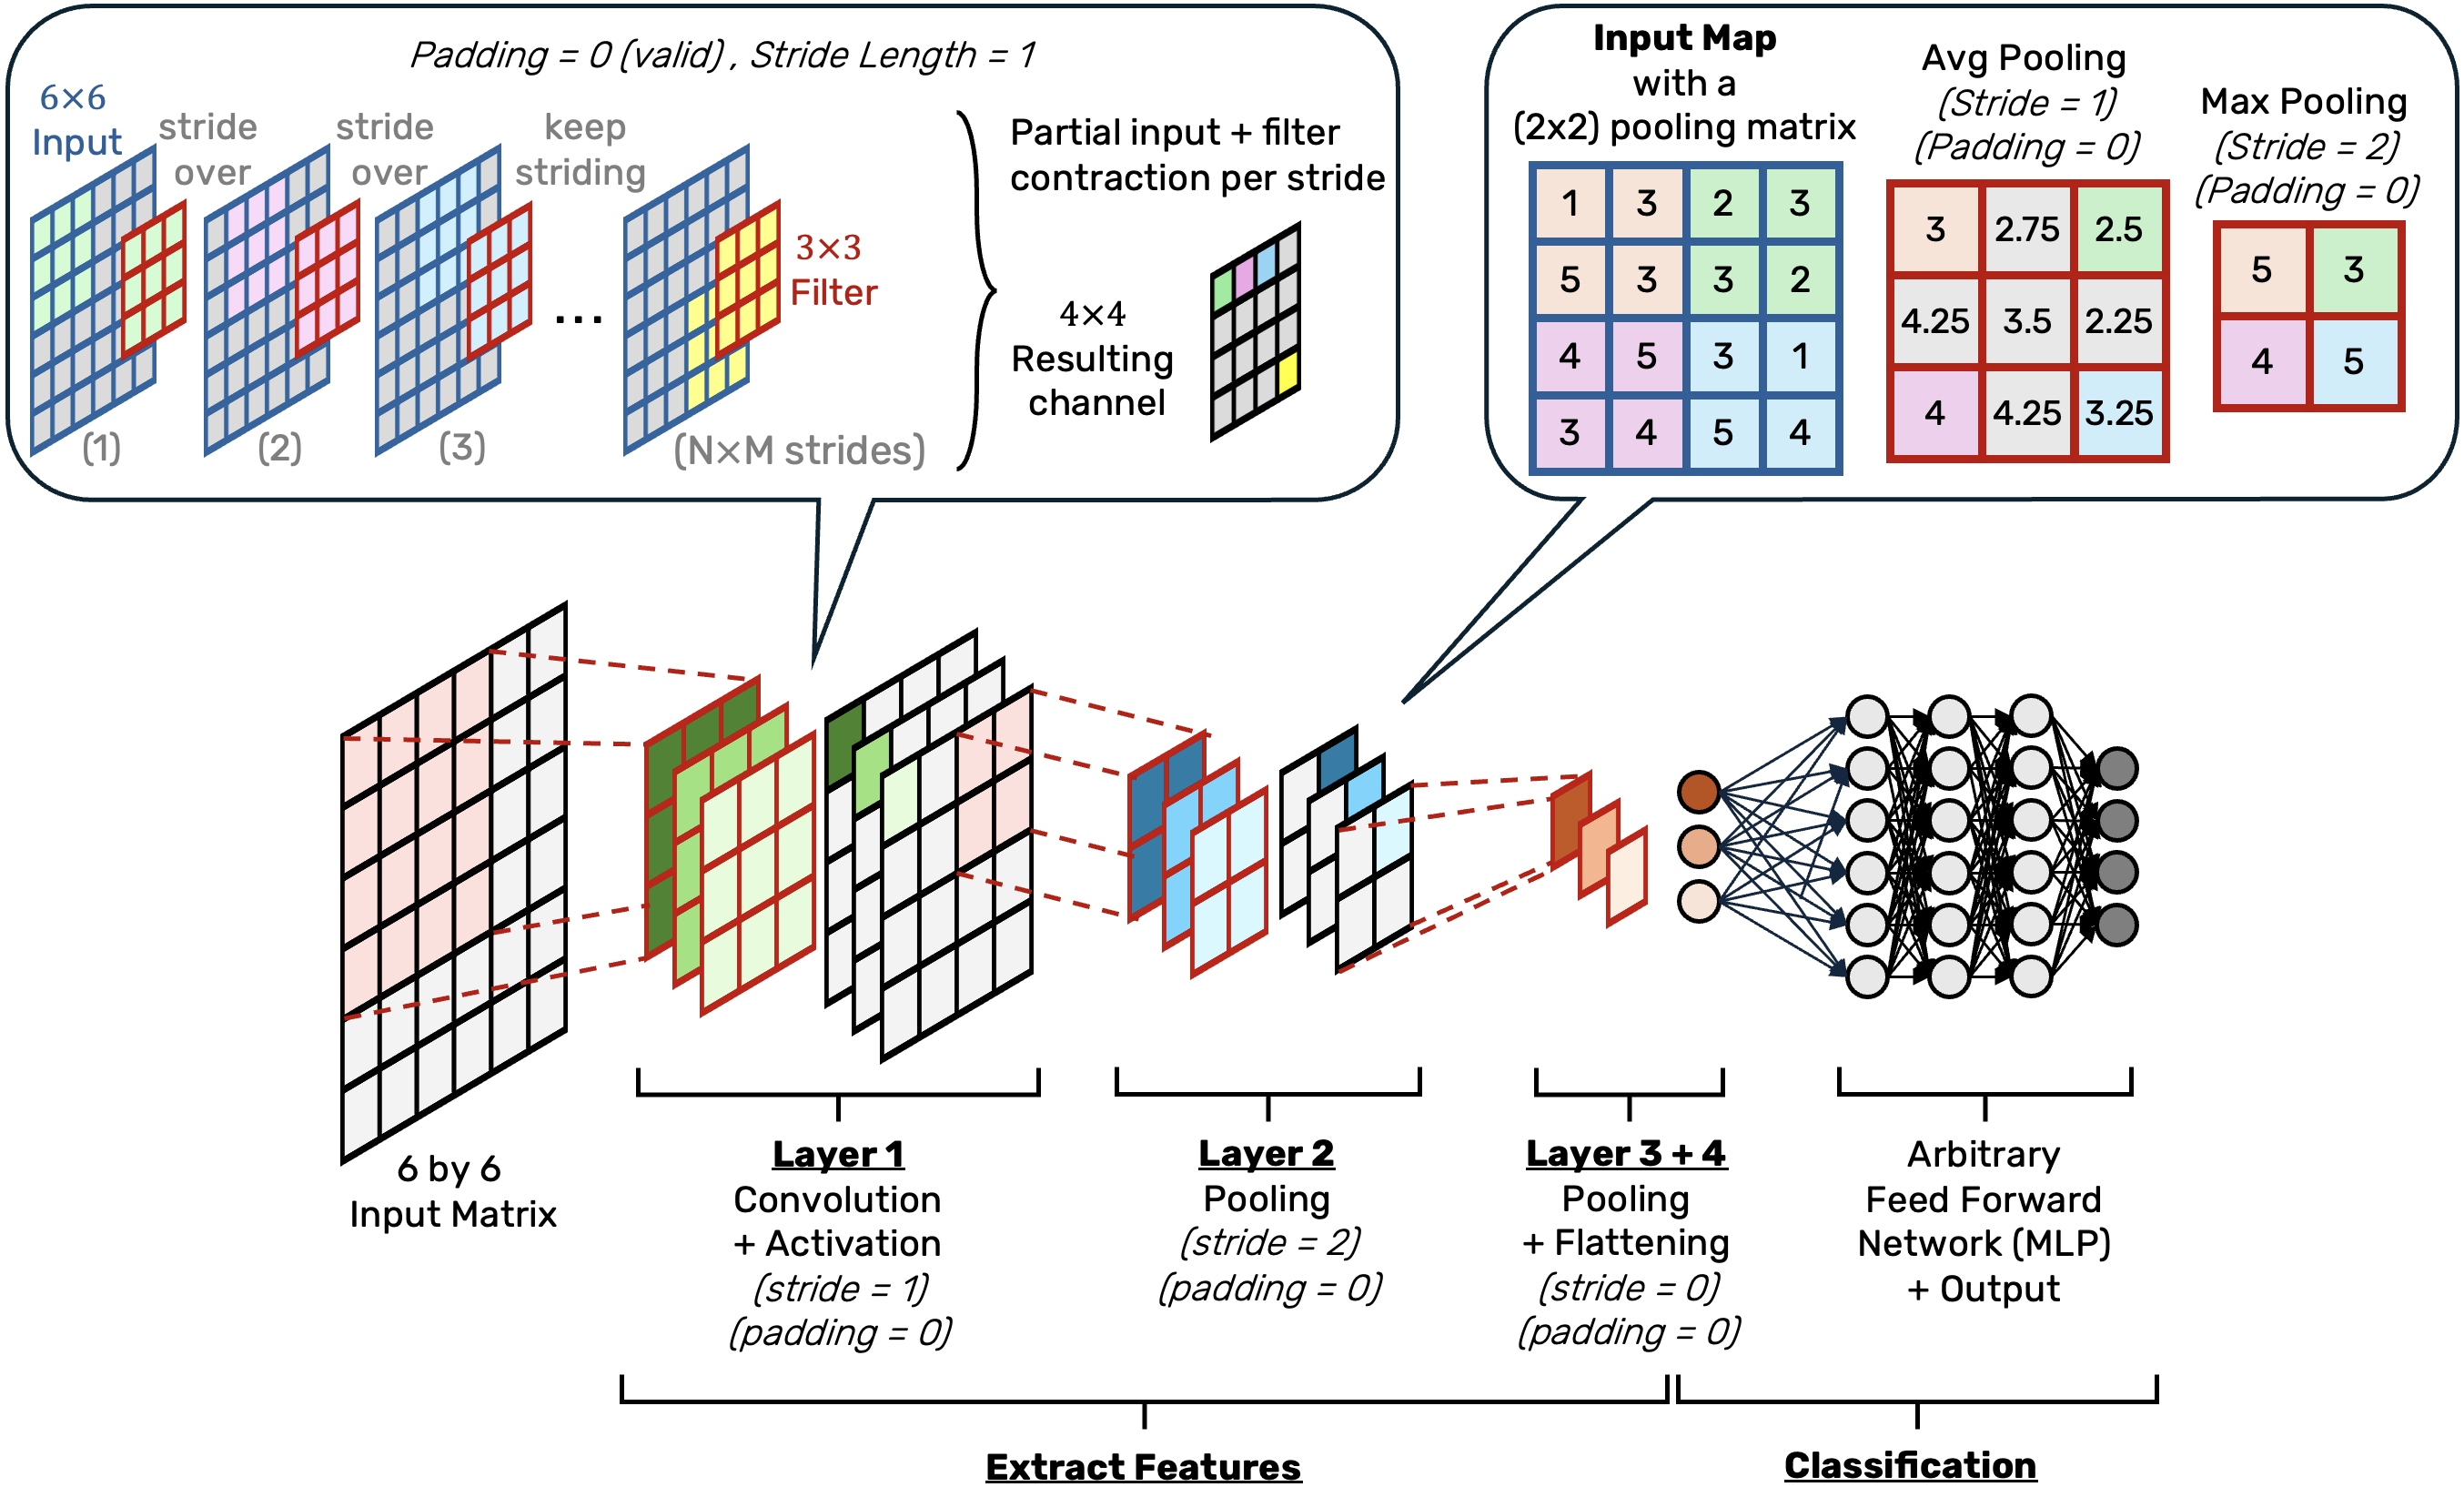
\includegraphics[width=\linewidth]{figures/cnn_schematic.png}
    \caption{Schematic of a CNN with one convolution layer and two pooling layers. The kernels in layer one and two have three filters. The MLP after layer four is of any arbitrary shape and used for classification. The operation for applying a $3\times3$ convolution kernel made of three filters is shown in the top left message box. The operation of applying a $2\times2$ pooling matrix for both average and max pooling is shown in the top right message box. The resulting matrix of these operations is called a channel. Layer one would have three resulting channels.}
    \label{fig:cnn_schematic}
\end{figure}

\section{Software Description}
Figure \ref{fig:codejenn_flowchart} illustrates the workflow of \textsc{CodeJeNN}. The process begins with the user obtaining data to train a neural network. That data is used to train a model using Keras, and then its parameters and hyperparameters are saved in a .keras or .h5 file. The user then utilizes that file through \textsc{CodeJeNN} to generate self-contained C\texttt{++} code that reproduces the trained neural network. The main principle of CodeJeNN is to inline as much as possible, minimize external dependencies, execute efficiently on local hardware, and remain fully self-contained using internal implementations.

\begin{figure}[h!]
    \centering
    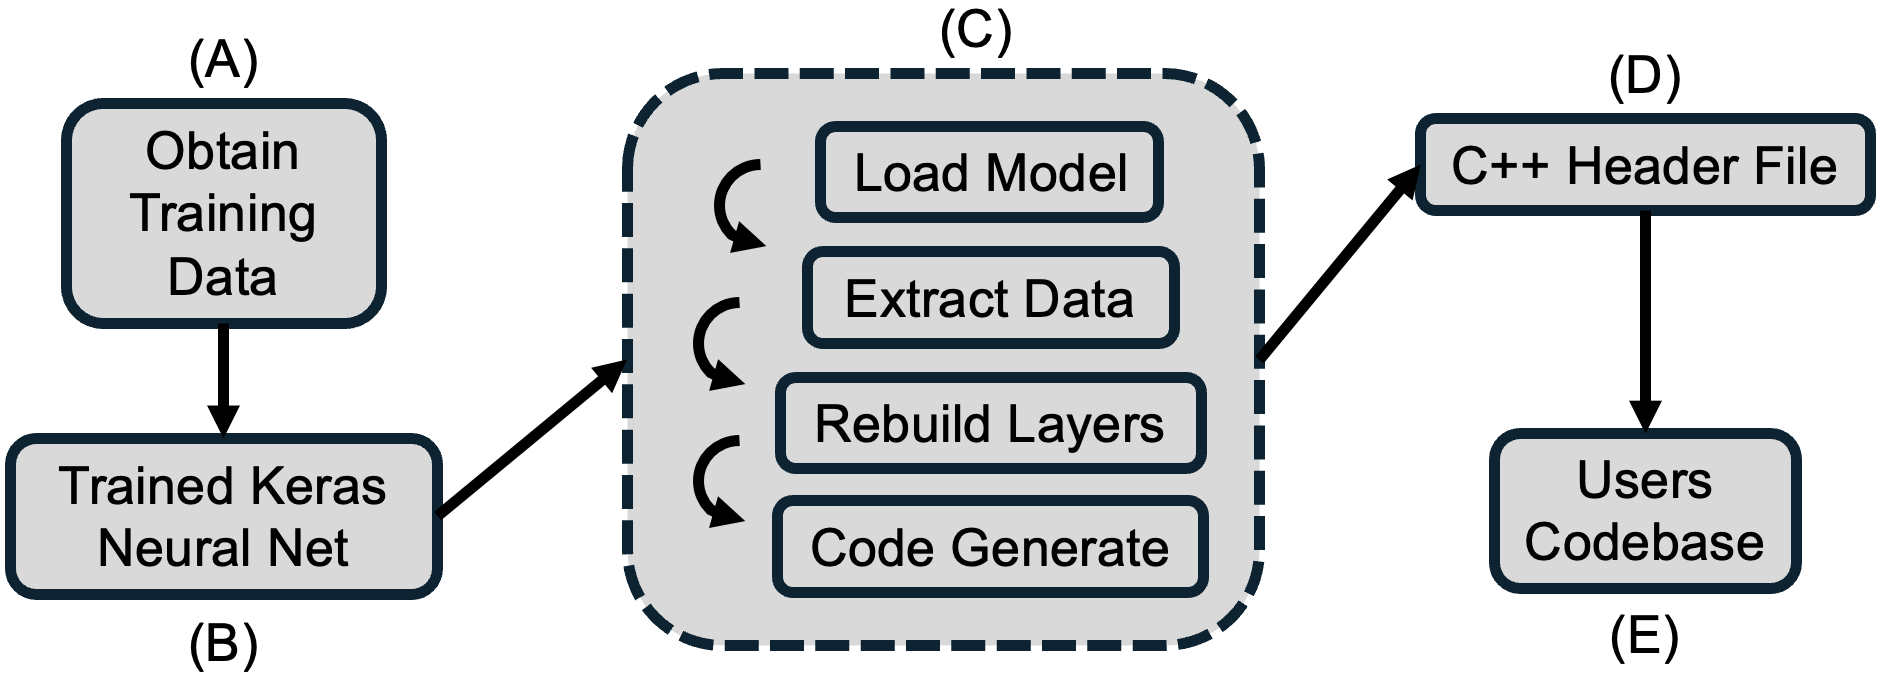
\includegraphics[width=.5\linewidth]{figures/codejenn_flowchart.png}
    \caption{\textsc{CodeJeNN} (C) code generates a \textsc{Keras}-trained neural network into a C\texttt{++} header file for the user's computational physics solver (E).}
    \label{fig:codejenn_flowchart}
\end{figure}

\subsection{Keras Compatibility}
Keras is chosen for its high-level API and backend integration with major frameworks (JAX, TensorFlow, PyTorch). It stores model architecture, hyperparameters, and parameters in a single file, allowing simplified model exchange and downstream \textsc{CodeJeNN} code generation. Its emphasis on readability and accessibility is important for researchers who wish to train models and automatically generate equivalent C\texttt{++} code without having to develop infrastructure in their codebase to allow for model inference.

\subsection{Code Generation}
\textsc{CodeJeNN}'s code generation proceeds in four steps: (1) load the saved model file using Keras' \verb|load_model| function, including any custom activation functions; (2) extract model parameters into a Python dictionary, where users can extend support for additional layers; (3) reconstruct the model from input to output layer; and (4) convert to a C\texttt{++} header file.

Algorithm \ref{alg:mlp_structure_example} presents a step-by-step procedure for how \textsc{CodeJeNN} formats a generated MLP once the model is loaded in Python. First, the propagation step functions (similar to the neuron edges shown in Figure \ref{fig:mlp_schematic}) are defined before the MLP function header. Then, within the MLP function body, there are three main sections. First, each layer’s parameters are generated. Second, the activation functions are defined as C\texttt{++} lambda functions. Third, the propagation step function calls are produced, where inference is performed. \textsc{CodeJeNN} generates neural networks in this format to enable downstream code optimization for users, where the propagation step functions benefit the most from modifications.

\begin{algorithm}[h]
\caption{Example of a code-generated MLP}
\begingroup
\makeatletter
\renewcommand{\alglinenumber}[1]{\makebox[1.5em][r]{\scriptsize #1}\hspace{1em}}
\makeatother

\begin{algorithmic}[1]
\vspace{0.5\baselineskip}
\State \textbf{Import packages:} iostream, array, cmath, functional, etc.

\vspace{0.5em}
\State \textbf{Define propagation step functions:}
\State \hspace{1em} Dense(outputs, inputs, weights, biases, input size, activation)
\State \hspace{1em} UnitNormalization(outputs, inputs, epsilon)

\vspace{0.5em}
\Function{MLP}{input}
    \State \textbf{Print model parameters:}
    \State \hspace{1em} Layer weights and biases
    \State \hspace{1em} Filter parameters
    \State \hspace{1em} Input/Output normalization constants

    \vspace{0.5em}
    \State \textbf{Define lambda activation functions:}
    \State \hspace{1em} linear(input)
    \State \hspace{1em} gelu(input)
    \State \hspace{1em} custom\_activation(input, index)

    \vspace{0.5em}
    \State \textbf{Propagation step:}
    \State \hspace{1em} Normalize $x \leftarrow (x - \mu_{in}) / \sigma_{in}$
    \State \hspace{1em} $h_1 \leftarrow \text{Dense}(x, W_1, b_1, linear)$
    \State \hspace{1em} $h_2 \leftarrow \text{UnitNormalization}(h_1, \epsilon)$
    \State \hspace{1em} $h_3 \leftarrow \text{gelu}(h_2)$
    \State \hspace{1em} $h_4 \leftarrow \text{Dense}(h_3, W_4, b_4, linear)$
    \State \hspace{1em} $h_5 \leftarrow \text{custom\_activation}(h_4)$
    \State \hspace{1em} Denormalize: $y \leftarrow h_5 \cdot \sigma_{out} + \mu_{out}$
    \State \Return $y$
\EndFunction
\vspace{0.5\baselineskip}
\end{algorithmic}
\endgroup
\label{alg:mlp_structure_example}
\end{algorithm}

\subsection{Algorithm Design Structure}
\label{sec:alg_struct_specs}
The generated code is written such that everything is known at compile time, allowing efficient cache utilization and fast inlined computation. As a result, an important design choice is the explicit use of syntax-level specifications, such as \texttt{void}, \texttt{inline}, \texttt{constexpr}, and \texttt{static}, which are applied consistently across arrays, headers, and function templates. Because minimizing computational cost is the top priority, \textsc{CodeJeNN} aggressively inlines generated code wherever possible.

Most computational physics codes are already highly optimized, and further aggressive optimization of the generated code from \textsc{CodeJeNN} prior to integration can be counterproductive. For example, nested parallelism arising from both the neural network and its evaluation can lead to thread oversubscription and degraded performance, where more threads are launched than available hardware resources \cite{yan_proposal_2016}. As a result, compile-time optimizations and the use of external libraries are intentionally deferred to the user to explore. The objective is to achieve readable and accessible neural networks which can be manipulated even further once their implementation is satisfactory. This design choice also motivates placing propagation step functions at the top of the generated models (Algorithm~\ref{alg:mlp_structure_example}), where they are most amenable to user-directed optimization. In addition, loops within lambda-based activation functions and lower-level function calls are structured to allow straightforward parallelization or vectorization when appropriate.

\subsection{Capabilities and Limitations}
\textsc{CodeJeNN} supports the following activation functions

\begin{multicols}{4}
\raggedcolumns 
    \begin{itemize}[itemsep=-5pt, topsep=0pt, leftmargin=*]
        \item[] \textsc{ReLU} \cite{nair_rectified_2010}
        \item[] \textsc{Sigmoid}
        \item[] \textsc{Tanh}
        \item[] \textsc{LeakyReLU} \cite{he_delving_2015}
        \item[] \textsc{Linear}
        \item[] \textsc{ELU} \cite{clevert_fast_2016}
        \item[] \textsc{Swish} \cite{ramachandran_searching_2017}
        \item[] \textsc{SiLU} \cite{ramachandran_searching_2017}
        \item[] \textsc{GeLU} \cite{hendrycks_gaussian_2023}
        \item[] \textsc{Softmax}
        \item[] \textsc{Mish} \cite{misra_mish_2020}
        \item[] \textsc{Softplus} \cite{dugas_incorporating_2000}
    \end{itemize}
\end{multicols}

\noindent 
\textsc{CodeJeNN} also supports custom activation functions by requiring users to (1) serialize the custom function when saving their model, and (2) define it in a Python script when loading. Examples are provided in the tutorials. Normalization parameters for inputs and outputs are also supported.

\textsc{CodeJeNN} supports the following layers from the \textsc{Keras} layer API \cite{chollet_keras_2015}:
\setlength{\columnsep}{-5em}
\begin{multicols}{2}
\begin{itemize}[itemsep=-5pt, topsep=0pt, leftmargin=*]
    \item[] \textsc{Dense}
    \item[] \textsc{Pure Activation}
    \item[] \textsc{Dropout}
    \item[] \textsc{1D, 2D, 3D Spatial Drop} \cite{tompson_efficient_2015}
    \item[] \textsc{Reshape}
    \item[] \textsc{Flatten}
    \item[] \textsc{Rescale}
    \item[] \textsc{Layer Normalization}
    \item[] \textsc{Batch Normalization}
    \item[] \textsc{Group Normalization}
    \item[] \textsc{Unit Normalization}
    \item[] \textsc{1D, 2D, 3D Convolution}
    \item[] \textsc{1D, 2D, 3D Transposed Conv} \cite{dumoulin_guide_2018, zeiler_deconvolutional_2010}
    \item[] \textsc{1D, 2D Depthwise Convolution}
    \item[] \textsc{1D, 2D Separable Convolution}
    \item[] \textsc{1D, 2D, 3D Max Pooling}
    \item[] \textsc{1D, 2D, 3D Average Pooling}
    \item[] \textsc{1D, 2D, 3D Global Max Pooling}
    \item[] \textsc{1D, 2D, 3D Global Average Pooling}
\end{itemize}
\end{multicols}

There are limitations to \textsc{CodeJeNN}. The primary limitation is that \textsc{CodeJeNN} only supports single-branch neural networks. The model operates on a single input dataset and does not allow multiple independent datasets; however, this input dataset may be of arbitrary dimensionality. A secondary limitation is the number of configuration options within a layer that \textsc{CodeJeNN} can support. For instance, in the Keras 3 API documentation \cite{chollet_keras_2015}, a 3D transposed convolution layer allows users to specify different regularizer options, which are not supported by \textsc{CodeJeNN}. Because the code-generation pipeline supports only a subset of these configurations, users are directed to the source-code tutorials for full details.

To support development and integration, \textsc{CodeJeNN} also includes a debugging API. \textsc{Keras} has a \texttt{model.summary()} function for a trained and loaded model that provides a tabulated summary of the network architecture and layer dimensions. After code generation, \textsc{CodeJeNN} compares what is extracted from that model against what \texttt{model.summary()} provides. Additionally, even when the C\texttt{++} model generates successfully, there can still be logic/algebraic errors when performing inference. With the debug flag on, \textsc{CodeJeNN} inserts print statements at the end of each layer, displaying the first ten output values of that layer. This allow pinpointing errors layer differences within a model. In practice, the majority of issues arise from user-defined custom activation functions, where the Python implementation of a custom activation does not match its C\texttt{++} counterpart.

We have also considered variadic templates as an alternative to for loops. However, such templating would quickly increase compilation time, code size, and memory usage. For instance, consider an MLP with an input sample size of $1\times 400$ and a first hidden layer of $256$ neurons. This configuration would require $102{,}400$ weights in the first layer alone, making a fully templated implementation impractical. Consequently, this approach does not scale well to very large models due to the rapid growth in memory and compilation costs, which represents a significant limitation. For many physics applications, this limitation is acceptable because deployed models are intentionally kept small and efficient to satisfy hardware and real-time constraints. \textsc{CodeJeNN}’s aggressively inlined code generation is well suited to these use cases, where memory and computational costs must be considered across the entire numerical workflow and models are typically kept compact to conserve CPU time, memory, and computing-node resources. If a generated model exceeds the available hardware memory, computational costs can increase substantially, leading to inefficient execution. In practice, however, large models are often unnecessary for accurate inference in scientific computing applications. Instead, predictive performance is frequently influenced more by factors such as data preprocessing, sampling strategies, and feature representation than by increases in model size alone \cite{zhang_multi-scale_2022}.

\section{Illustrative Examples}
We demonstrate the computational performance and implementation of \textsc{CodeJeNN} via two test cases. First, we show the total wall-clock inference time of \textsc{CodeJeNN} and Keras with an MLP and CNN. This is conducted on an Apple MacBook M1 Pro, with an M1 Pro chip containing 32 GB of memory and 10 cores (2 efficiency and 8 high-performance with peak performance of 3.22 GHz). Second, we apply a neural network implementation to replace the viscosity model in a simulation of a two-dimensional subsonic splitter-plate mixing layer. This is conducted on a compute cluster using a single node equipped with two AMD EPYC 7702 64-Core processors and 270 GB in memory.


% CPU(s):              256
% On-line CPU(s) list: 0-255
% Thread(s) per core:  2
% Core(s) per socket:  64
% Socket(s):           2
% NUMA node(s):        8
% Vendor ID:           AuthenticAMD
% CPU family:          23
% Model:               49
% Model name:          AMD EPYC 7702 64-Core Processor
% Stepping:            0
% CPU MHz:             3349.759
% CPU max MHz:         2183.5930
% CPU min MHz:         1500.0000


\subsection{Inference Speed}
In our first test case, we compare the inference performance of both an MLP and CNN created in Keras and code-generated by \textsc{CodeJeNN}. Keras requires a backend deep learning framework providing C\texttt{++} API and tensor operations, such as \textsc{TensorFlow}, \textsc{PyTorch}, or \textsc{JAX}. To ensure fair comparison, all models are tested on a single CPU core using a single thread. Since \textsc{PyTorch} and \textsc{TensorFlow} are the most widely used frameworks, only these two backends are evaluated. By default, \textsc{TensorFlow} converts a model into graph mode by tracing hierarchical operations and executing them efficiently. \textsc{PyTorch} defaults to eager execution. Keras also allows Just-in-Time (JIT) compilation, which compiles the computational graph into optimized C\texttt{++} code. TensorFlow uses Accelerated Linear Algebra (XLA) compilation, whereas PyTorch utilizes TorchDynamo, AOTAutograd, and the Inductor compiler backend. These frameworks aggressively fuse operations, reduce memory usage, and apply target-specific optimizations. All Keras models are evaluated in eager mode with JIT compilation disabled to ensure fair baseline comparison. For completeness, we report JIT-compiled times to demonstrate performance achievable with aggressive backend optimization and provide a useful target for optimizing the generated C\texttt{++} models.

Table \ref{tab:mlp_inference} shows inference performance of \textsc{CodeJeNN} compared to Keras for two 64-bit models, an MLP and CNN using 10,000 random data samples. Data samples are preloaded before benchmarking. The inference process performs a dry-run with a single sample to initialize system resources and cache, then measurements are taken over 10,000 iterations. 
\begin{table}[h]
    \centering
    \begin{tabular}{r @{\hspace{3em}} c c c}
        \makecell[r]{Deep Learning\\Library} 
        & \makecell{MLP\\Inference (sec)} 
        & \makecell{CNN\\Inference (sec)} 
        & \makecell{Unbounded Memory\\ CNN Inference (sec)} \\
        \noalign{\vskip 3pt}
        \hline
        \noalign{\vskip 3pt}
        Keras (TensorFlow)      & $12.01 \pm 0.24$          & $19.14 \pm 0.29$          & $21.36 \pm 0.38$ \\
        Keras (PyTorch)         & $18.20 \pm 0.19$           & $26.77 \pm 1.13$          & $27.53 \pm 0.48$ \\
        Keras (JIT-TensorFlow)  & $1.21 \pm 0.03$           & $2.17 \pm 0.18$           & $\mathbf{3.60} \pm 0.05$ \\
        Keras (JIT-PyTorch)     & $4.33 \pm 0.29$           & $7.75 \pm 0.31$           & $8.47 \pm 0.16$ \\
        \textsc{CodeJeNN}       & $\mathbf{0.48} \pm 0.01$  & $\mathbf{1.05} \pm 0.01$  & $10.75 \pm 0.23$
    \end{tabular}
    \caption{MLP and CNN inference. The inference times represent the total wall-clock time to compute the inference of 10,000 random data samples sequentially for an MLP, CNN, and an unbounded memory CNN, created by Keras and \textsc{CodeJeNN}. We test the Keras backend inference speed of \textsc{PyTorch} and \textsc{TensorFlow} and their JIT compilation optimization. Each inference case is tested three times to ensure precision.}
    \label{tab:mlp_inference}
\end{table}

We use an MLP architecture with a 1,000-dimensional input passed through a 64-neuron dense layer with \textsc{ReLU}, Batch Normalization, and 0.3 Dropout, followed by a 32-neuron \textsc{ReLU} layer and a 100-neuron sigmoid output. The network is trained using Adam optimizer and binary cross-entropy loss on 10,000 randomly generated, standardized samples. Our CNN contained a $10\times100\times1$ input, passed through convolutional layers (8 filters, $3\times3$, softplus; 16 filters, tanh), a $3\times3$ transposed convolution with \textsc{ReLU}, flattened into a 32-neuron Mish layer, and 100-neuron softmax output. The CNN is trained with Adam optimizer and sparse categorical cross-entropy loss. To test \textsc{CodeJeNN} capabilities, we ensured each layer utilized different tensor operations.

Inference in \textsc{CodeJeNN} executes roughly 25 times faster than Keras using a \textsc{TensorFlow} backend and achieves nearly 38 times speedup with \textsc{PyTorch}. When optimized with JIT compilation, \textsc{CodeJeNN} remains roughly 2.5 times and 9 times faster than \textsc{TensorFlow}'s and \textsc{PyTorch}'s JIT versions, respectively. For CNNs, speedup factors are smaller but substantial: approximately 18 times and 26 times relative to standard Keras for \textsc{TensorFlow} and \textsc{PyTorch}, and 2 times and 7 times faster than their JIT-compiled counterparts.

The third column in Table \ref{tab:mlp_inference} shows the results of evaluating a larger CNN architecture where the filters in the \textit{Conv2DTranspose} layer are increased to 32 and the subsequent \textit{Dense} layer is expanded to 64 neurons. The table shows that these architectural changes caused a significant increase in inference cost, as the number of floating-point operations required for those layers scaled quadratically. This expansion causes the model to transition from being compute-bound to memory-bound, as the larger weight matrices exceed the hardware's L1 and L2 cache capacities and saturate available memory bandwidth. This results in high-latency stalls as the CPU waits for weight data from main memory. Although these memory limitations are inherent to larger neural network architectures, \textsc{CodeJeNN} generates standalone, dependency-free C\texttt{++} source code that users can modify and optimize directly for their target hardware.

\subsection{Inference Demonstration on a Splitter Plate}
We embedded a neural network to replace viscosity in a hydrogen-air splitter-plate mixing layer simulation using \textsc{OpenFOAM} \cite{weller_tensorial_1998} and \textsc{DetonationFOAM} \cite{sun_detonationfoam_2023}. The demonstration targets mixture-averaged viscosity computed with Wilke's mixing rule \cite{wilke_viscosity_1950}. While viscosity evaluation is typically a minor cost in chemically reacting flow solvers, this case demonstrates that neural networks can be robustly embedded within a CFD workflow.

In the baseline case, the mixture dynamic viscosity is calculated from species-dependent viscosity fits and mole fractions as
%
\begin{equation}
\mu_{\mathrm{mix}}
=
\sum_{i=1}^{N}
\frac{X_i \mu_i}
     {\sum_{j=1}^{N} X_j \Phi_{ij}}
\label{eq:wilke}
\end{equation}
%
where $X_i$ is the mole fraction of species $i$, and the interaction coefficient is
%
\begin{equation}
    \Phi_{ij} =
    \frac{1}{\sqrt{8}}
    \left(1 + \frac{M_i}{M_j}\right)^{-1/2}
    \left[
        1 +
        \left(\frac{\mu_i}{\mu_j}\right)^{1/2}
        \left(\frac{M_j}{M_i}\right)^{1/4}
    \right]^2,
    \label{eq:phi}
\end{equation}
%
with $M_i$ the molar mass of species $i$. The species viscosity is evaluated using a log-polynomial fit in temperature:
%
\begin{equation}
    \mu_i =
    0.1\exp\!\left(
        A_{1,i}
        + A_{2,i}\ln T
        + A_{3,i}(\ln T)^2
        + A_{4,i}(\ln T)^3
    \right)
    \quad [\text{Pa$\cdot$ s}].
    \label{eq:muspecies}
\end{equation}
%
The domain is $15\,\text{mm}\times5\,\text{mm}\times0.2\,\text{mm}$. Two streams entered from the left and are separated at the centerplane at $y=2.5\,\text{mm}$:
%
\begin{itemize}
    \item \textbf{H$_2$ stream}: $M=0.3$, $T=350\,\text{K}$, $p=101{,}325\,\text{Pa}$,
    $U\approx427\,\text{m/s}$.
    \item \textbf{Air stream}: $M=0.3$, $T=1500\,\text{K}$, $p=101{,}325\,\text{Pa}$,
    $U\approx226\,\text{m/s}$.
\end{itemize}

The mesh consisted of two blocks per stream with $190 \times 60 \times 1$ cells each. Streamwise grading ranged from $20\,\mu\text{m}$ at the inlet to $200\,\mu\text{m}$ at the outlet, with wall-normal grading symmetric about the centerplane ($10\,\mu\text{m}$ at the shear interface, coarsening to $\approx 100\,\mu\text{m}$ at boundaries). The top, bottom, and right boundaries are prescribed as zero-gradient supersonic outflow.


\textsc{DetonationFOAM} uses mixture-averaged transport employing the Wilke mixing rule. Chemistry is disabled to reduce computational cost. A quasi-steady flow field after five flow-through times ($5 \times L/U_{x,air}\approx 3.32 \times 10^{-4}$~s) is shown in Figure~\ref{fig:cfd_domain}, where unsteady mixing layer structures grow with downstream distance. We replaced Wilke's model with a neural network mapping thermochemical state directly to viscosity: $\left(Y_{\mathrm{H}_2},Y_{\mathrm{O}_2},Y_{\mathrm{N}_2},T\right)\rightarrow\mu_{\text{mix}}$.

\begin{figure}[H]
    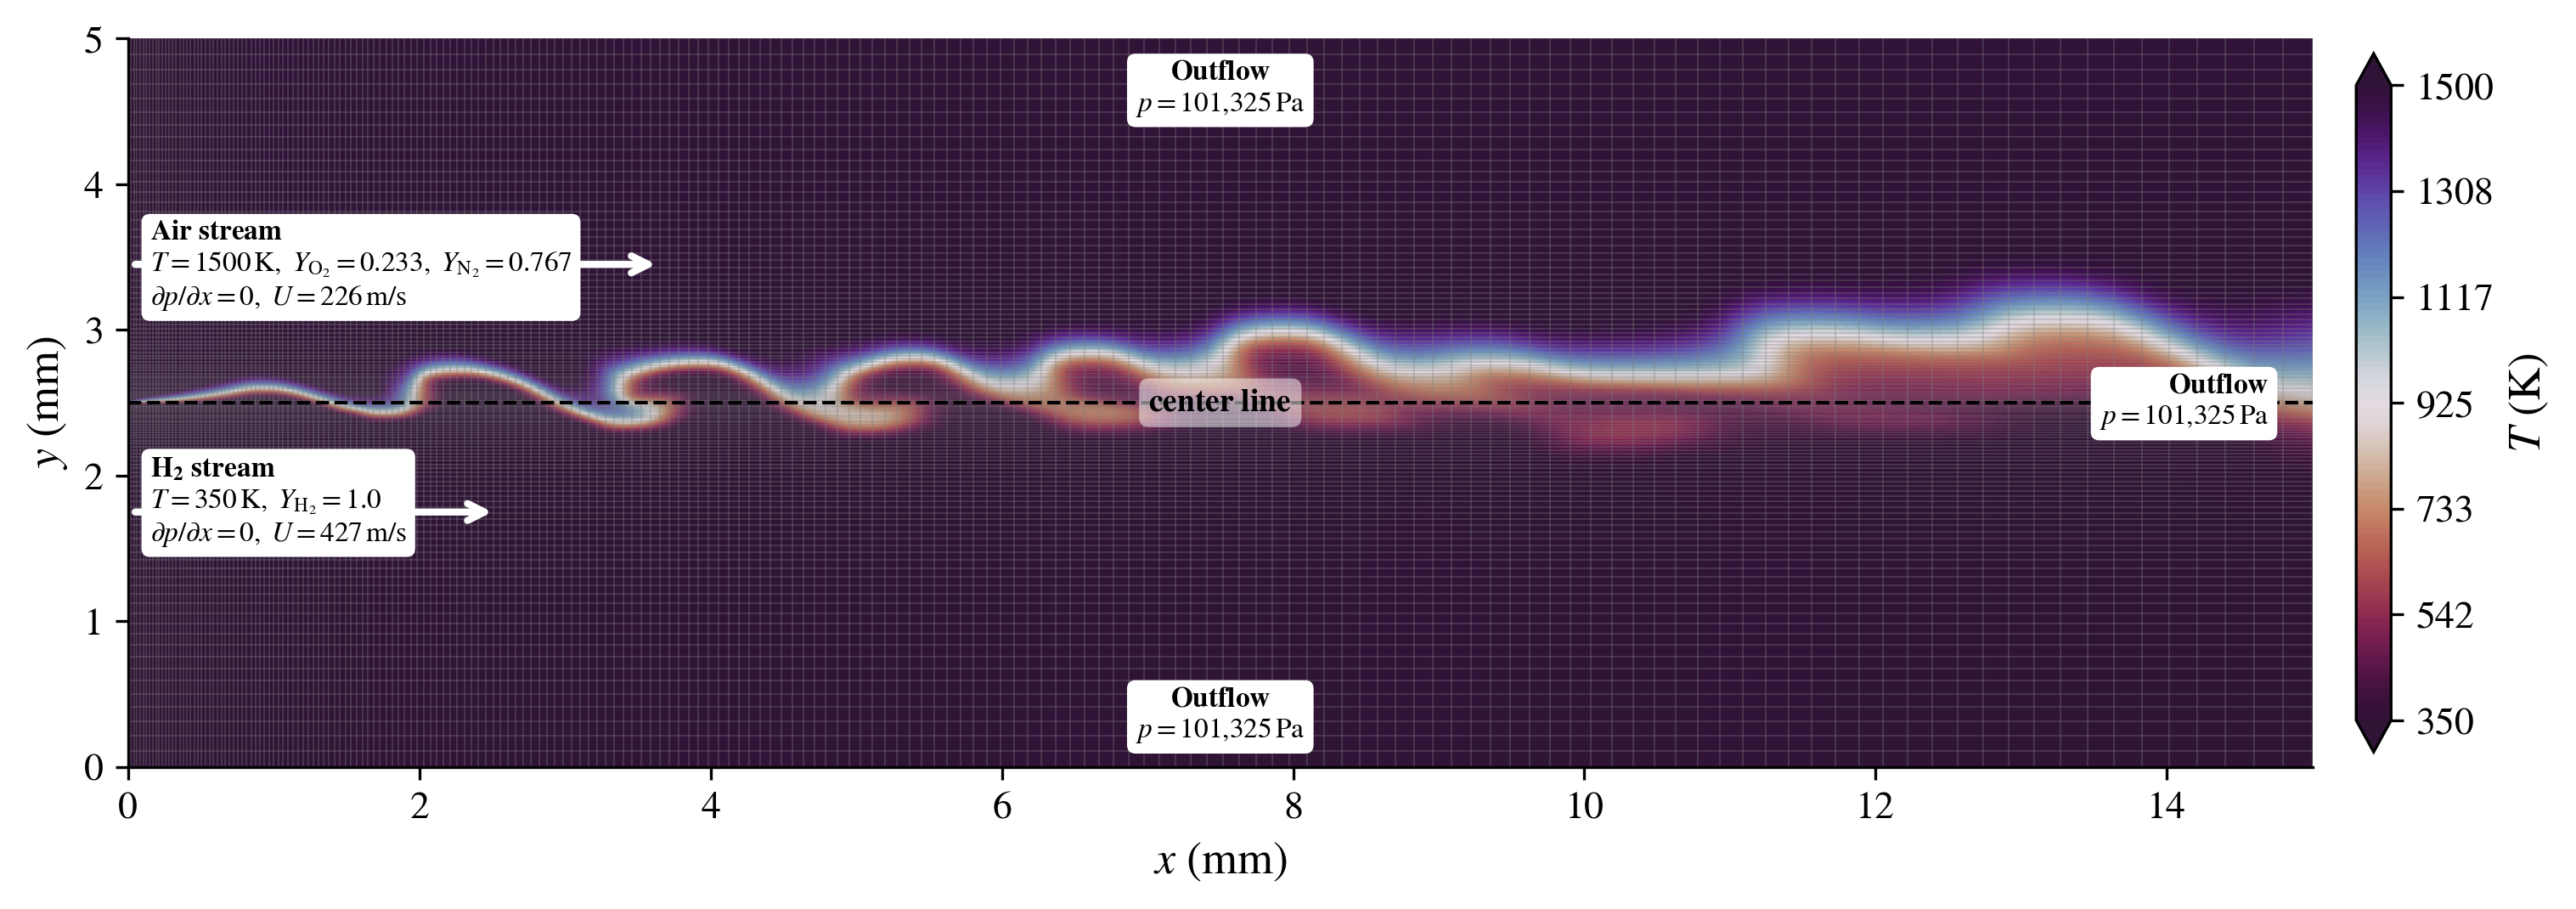
\includegraphics[width=\textwidth]{figures/temperature_field.png}
    \caption{Temperature and flow domain}
    \label{fig:cfd_domain}
\end{figure}

A fully-connected feed-forward neural network is generated using CodeJeNN and trained on $10^4$ random states $(Y_{H_2},Y_{O_2},Y_{N_2},T)$ generated from a small OpenFOAM utility, \texttt{generateData}, contained on the \textsc{CodeJeNN} repository that uses the \texttt{detonatFOAM} Wilke's rule (Eqs.~\eqref{eq:wilke}--\eqref{eq:muspecies}) as training target. The stratified distribution consisted of 60\,\% samples from a symmetric Dirichlet distribution with $Y_i\sim\mathcal{U}(0,1)$ and $T\sim\mathcal{U}(200,3000)$\,K, and 40\,\% along the physical mixing line,
\begin{equation}
    \mathbf{Y}(\alpha) = \alpha\,\mathbf{Y}_{\text{fuel}}
                       + (1-\alpha)\,\mathbf{Y}_{\text{ox}}, \quad
    \alpha\sim\mathcal{U}(0,1),
\end{equation}
where $\mathbf{Y}_{\text{fuel}}=(1,0,0)$ (pure H$_2$) and
$\mathbf{Y}_{\text{ox}}=(0,\,0.233,\,0.767)$ (air), with temperature
$T(\alpha)=\alpha T_{\text{fuel}}+(1-\alpha)T_{\text{ox}}+\delta T$,
$\delta T\sim\mathcal{U}(-200,200)$\,K, $T_{\text{fuel}}=350$\,K, and
$T_{\text{ox}}=1500$\,K. This importance-sampling strategy ensures coverage
of the pure-stream conditions that are underrepresented by the Dirichlet
distribution yet dominate the inlet regions of the splitter-plate domain.

The network uses 3 hidden layers with 12 neurons each (385 parameters total) and Tanh activation. Normalized inputs and de-normalized output are embedded directly in C\texttt{++} headers within a modified \textsc{DetonationFOAM} solver, requiring no external files at runtime. The network is verified against the Wilke model over 2\,000 randomly sampled states. The relative error for each sample is computed as
\begin{equation}
\epsilon = \frac{|\mu_{\text{Wilke}} - \mu_{\text{NN}}|}{\mu_{\text{Wilke}}}, \label{error}
\end{equation}
yielding a mean error of 0.12 and a maximum error of 8.12.

Two simulations are run for five more flow-through times: one using the native Wilke model and another using the embedded neural network. Figure~\ref{fig:u_error} presents the percent error for the $x$-direction velocity field, computed as $100\times\left|u_{x, Wilke}-u_{x, NN}\right|/u_{x, Wilke}$. The neural network introduces minimal error, reaching a maximum of 0.25\% only in the mixing layer. The absence of large-scale error structures elsewhere indicates that the neural-network viscosity model preserves overall flow evolution and instability development. These results demonstrate that CodeJeNN-generated networks can be embedded in CFD solvers as surrogates for constitutive models while maintaining close agreement with reference solutions.

\begin{figure}[H]
    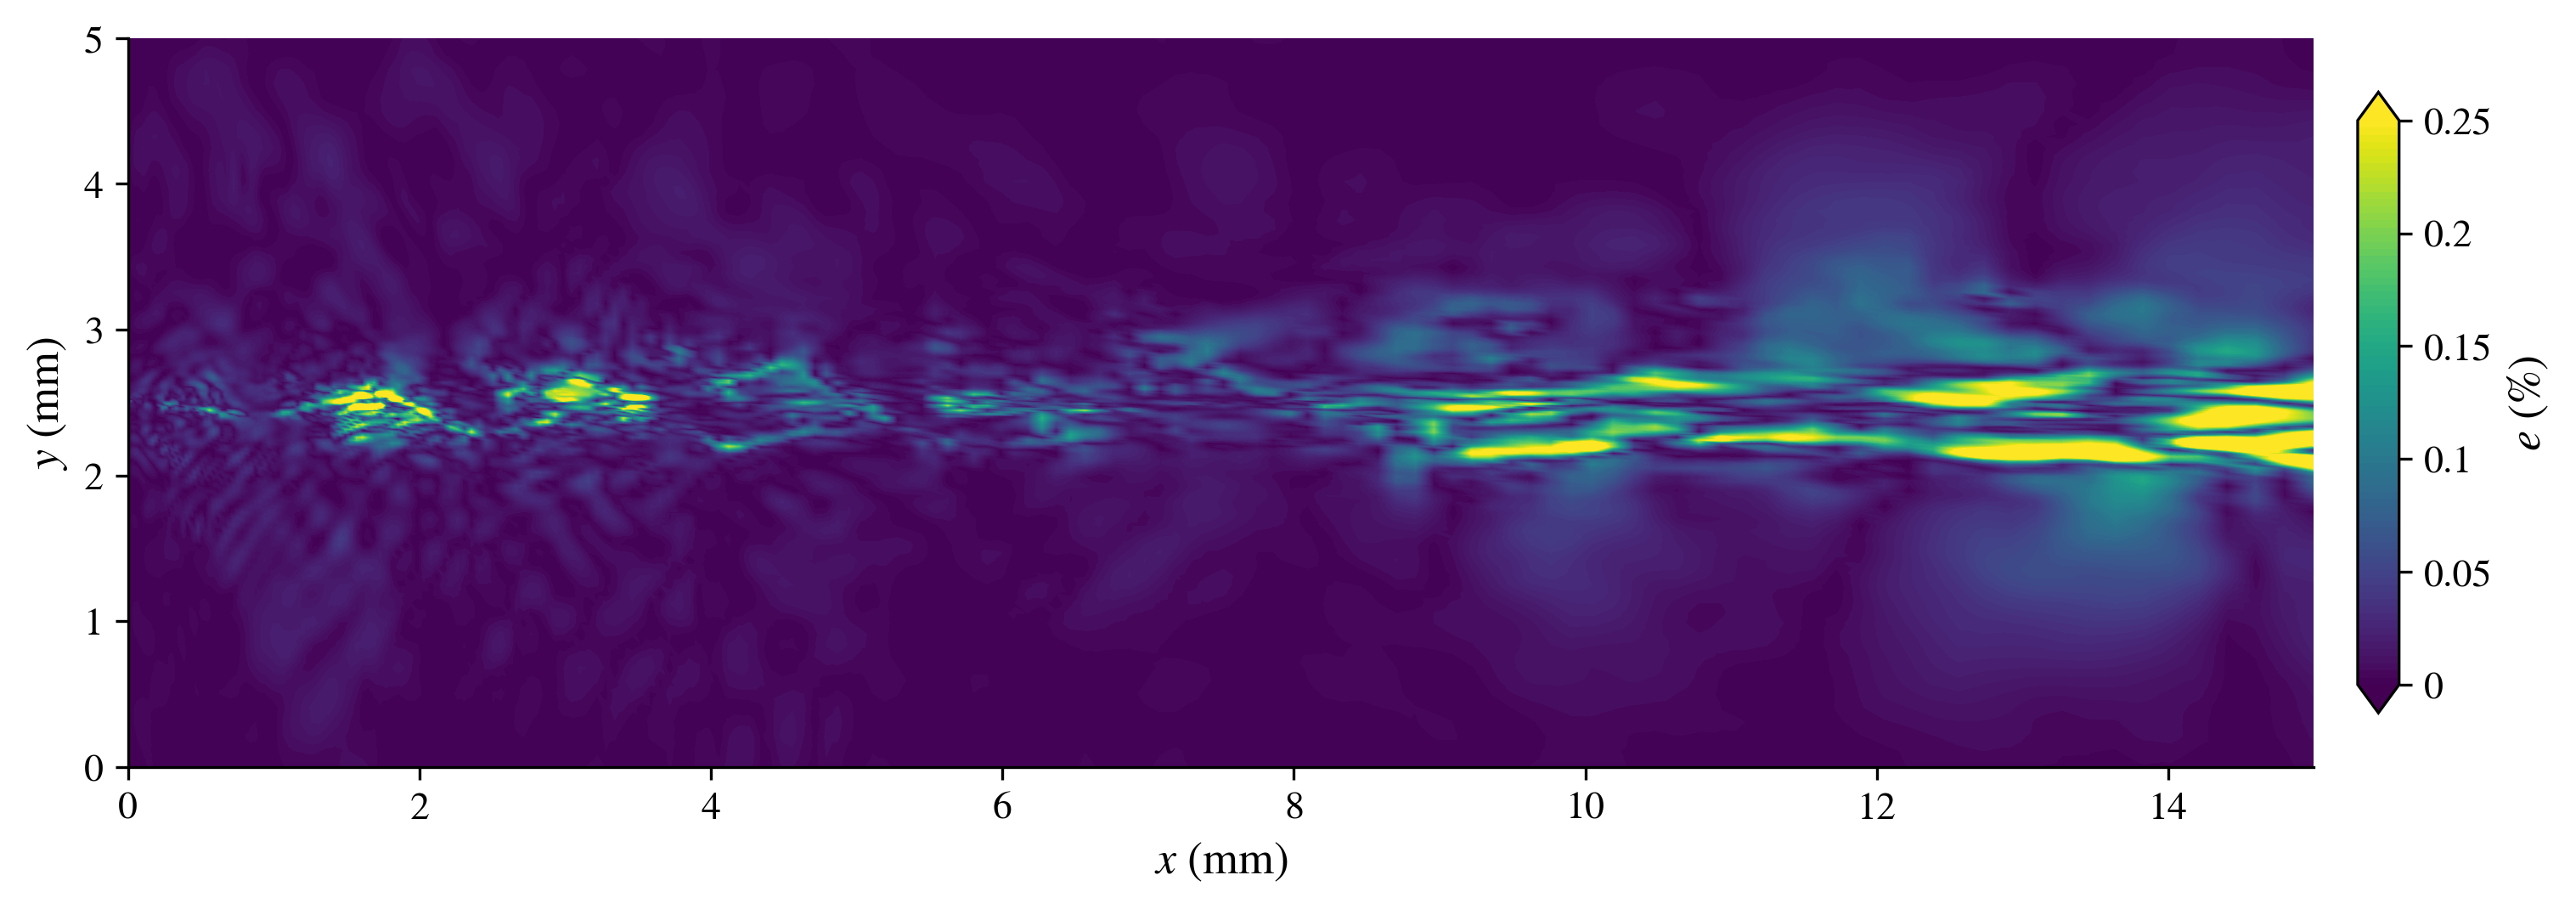
\includegraphics[width=\textwidth]{figures/Ux_error_pct_NN1.png}
    \caption{Error after one flow-through time}
    \label{fig:u_error}
\end{figure}

\section{Impact}
This software can allow researchers to integrate neural networks into their computational physics codebases with minimal additional infrastructure. Many physics experts may not wish to invest the time or resources to branch into machine learning solely to build code infrastructure. This product serves as a way to build inline infrastructure with only the prerequisite of a basic understanding of how neural networks perform inference. The key feature of \textsc{CodeJeNN} is its ability to produce raw source code where everything is inlined and enclosed within a single header file. This negates the need to worry about exporting tensor operations from high-performance libraries, since many computational physics codes utilize all available hardware. 

Integrating neural network inference into an established codebase using an LLM may require repeatedly supplying project-specific context and regenerating infrastructure whenever architectures change. Prior work has shown that software-engineering workflows can consume substantial token budgets, with context processing accounting for a large fraction of total token usage \cite{salim_tokenomics_2026}. By automatically generating self-contained inference code, CodeJeNN reduces reliance on repeated LLM-assisted infrastructure generation and the associated token costs. Additionally, it has been shown that LLM reasoning often contains redundant tokens that increase inference costs without providing proportional gains in performance \cite{han_token-budget-aware_2025}. \textsc{CodeJeNN} addresses this challenge by eliminating the need to repeatedly generate infrastructure code through an LLM, instead providing an easy-to-call function that computational physics practitioners can integrate directly while developing infrastructure on the fly.

Finally, \textsc{CodeJeNN} is designed to be extensible and repeatable. If a particular architecture does not exist within \textsc{CodeJeNN}, the way it is written allows a user to leverage an LLM to add the required logic with substantially fewer generated tokens. This enables a non-invasive workflow for generating new models while minimizing token consumption and reducing the effort required to experiment with new architectures. As a result, users can facilitate and implement neural network models within existing computational physics workflows in a shorter time period.

\section{Conclusion}
\textsc{CodeJeNN}, a C\texttt{++} neural network generation library, has been developed and demonstrated. This library is compatible with Keras, a commonly used deep learning API in computational physics, and enables users to implement neural networks in their codebases. The package does this by providing a self-contained C\texttt{++} rendition of the Keras model. This allows the user to optimize raw source code without performance bottlenecks. We have demonstrated \textsc{CodeJeNN} by replacing the viscosity model in a subsonic splitter-plate mixing layer simulation, along with evaluating its inference speed. 

Future work will integrate \textsc{Spektral} \cite{grattarola_graph_2020}, which is the GNN API for Keras that includes commonly used GNN layers such as message passing layers \cite{gilmer_neural_2017} and attention-based graphing layers \cite{thekumparampil_attention-based_2018}. Additionally, more activation functions will be added. We will also explore accelerating the inference performance of generated models by adding features to export functions using low-level high-performance libraries such as \textsc{Eigen} \cite{guennebaud_eigen_2010-1}. This path may also include using different data structures for model hyperparameters, allowing users to homogenize the neural network within their codebase. \textsc{CodeJeNN} is accessible at \url{https://github.com/jarcities/codejenn}.

\section{Conflict of Interest}
% Please select the appropriate text:

% Potential conflict of interest exists:
% We wish to draw the attention of the Editor to the following facts, which may be considered as potential conflicts of interest, and to significant financial contributions to this work. The nature of potential conflict of interest is described below: [Describe conflict of interest]

% No conflict of interest exists:
We wish to confirm that there are no known conflicts of interest associated with this publication and there has been no significant financial support for this work that could have influenced its outcome.


\section*{Acknowledgements}
\label{}

The authors wish to acknowledge Dr. Eric Marineau and Dr. Jonathan Sosa of the Hypersonic Aerothermodynamics, High-Speed Propulsion and Materials Program of the Office of Naval Research Code 35 for directly supporting this work.

\section*{Declaration of generative AI and AI-assisted technologies in the manuscript preparation process}
During the preparation of this work the author(s) used Claude from Anthropic in order to verify CFD test cases after infrastructure was already implemented. 
% Moreover, Google Gemeni was used to grammar check and improve clarity of certain sections of this manuscript. 
After using this tool/service, the author(s) reviewed and edited the content as needed and take(s) full responsibility for the content of the published article.


\bibliographystyle{elsarticle-num} 
\bibliography{References}

\end{document}
\endinput
%%
%% End of file `SoftwareX_article_template.tex'.
